\appendix

\section{Demo and Resources}
\label{sec:demo}

A live demo of the MemeSonic pipeline—including meme input, incongruity score visualization,
and synthesized audio playback—is available at:

\begin{center}
  \url{https://tinyurl.com/4schzjb5}
\end{center}

The demo allows users to upload a meme image with caption, inspect the per-modality emotion
distributions and computed incongruity score $\delta$, and listen to the three audio variants
(Vanilla TTS, Label-Guided, and MemeSonic).

Generated audio samples from our 100-meme evaluation set are available on Google Drive,
organized by sentiment class and voice setting:

\begin{center}
  \url{https://drive.google.com/drive/folders/1fuWLJP8FWZz0klj3jQmOCMFVCminqf46?usp=sharing}
\end{center}

% ─────────────────────────────────────────────────────────────────────────────
\section{Full Classification Results}
\label{sec:full_results}

Table~\ref{tab:full_acc} reports Accuracy (complementing the Macro-F1 in Table~\ref{tab:main_results})
across all methods and tasks. Table~\ref{tab:llm_vs_trained} and Figure~\ref{fig:llm_heatmap}
provide a direct Macro-F1 comparison between LLM zero-shot baselines and our best trained model
per task, isolating where each paradigm has an advantage.

\begin{table}[h]
\centering
\caption{Accuracy across all methods and tasks. Format mirrors Table~\ref{tab:main_results}.
\best{Bold green} = best trained model; LLM baselines shown for reference.}
\label{tab:full_acc}
\resizebox{\textwidth}{!}{%
\begin{tabular}{llccccccc|ccccc}
\toprule
 & & \multicolumn{7}{c|}{\textbf{Trained Models}} & \multicolumn{5}{c}{\textbf{LLM Zero-Shot}} \\
\cmidrule(lr){3-9}\cmidrule(lr){10-14}
Dataset & Task & Uni-I & Uni-T & Concat & Late & Incong & MULT & MMOE
        & GPT-4o & Gemini & o4-mini & Gemini-CoT & Qwen3 \\
\midrule
MET-Meme & intention  & 40.3 & 38.5 & 40.1 & 39.8 & 28.1 & 36.2 & 34.7
                      & 44.6 & 42.9 & \textbf{56.0} & 37.1 & 52.0 \\
MET-Meme & sentiment  & 29.4 & 28.2 & 36.8 & 33.1 & 30.5 & 29.0 & 31.9
                      & 33.6 & 38.8 & 39.6 & 45.9 & 35.9 \\
MET-Meme & hate       & \best{87.1} & 85.4 & 83.7 & 84.9 & 83.2 & 85.6 & 85.6
                      & 72.7 & 79.4 & 81.7 & 72.1 & 74.6 \\
MET-Meme & metaphor   & 81.2 & 75.5 & 82.9 & 81.8 & \best{87.6} & 84.7 & \best{87.6}
                      & 36.7 & 71.3 & 73.1 & 63.5 & 57.1 \\
\midrule
Memotion & humour     & 53.9 & 51.4 & 53.4 & \best{54.3} & 45.8 & 52.0 & 46.9
                      & 43.1 & 49.3 & 48.0 & 38.3 & 50.9 \\
Memotion & sarcasm    & \best{55.7} & 55.2 & 52.4 & 54.9 & 46.1 & 49.8 & 47.3
                      & 46.6 & 58.6 & 63.1 & 58.3 & 67.0 \\
Memotion & offensive  & 50.6 & 48.7 & 53.1 & 54.8 & 55.3 & 42.1 & \best{56.0}
                      & 42.1 & 50.2 & 76.4 & 49.3 & 46.3 \\
Memotion & motivational & 67.1 & 66.3 & 65.9 & \best{69.3} & 60.8 & 62.9 & 61.7
                        & 54.9 & 55.0 & 55.1 & 54.7 & 55.0 \\
Memotion & sentiment  & 57.3 & 55.9 & 56.8 & 56.5 & 49.4 & \best{62.7} & 50.3
                      & 50.1 & 45.7 & 50.8 & 43.9 & 40.0 \\
\midrule
MMSD 2.0 & sarcasm    & 77.5 & 77.6 & 82.6 & 82.0 & \best{84.0} & 83.0 & \best{84.0}
                      & 80.0 & 85.9 & 84.0 & 74.0 & 57.2 \\
\bottomrule
\end{tabular}}
\end{table}

\begin{figure}[h]
  \centering
  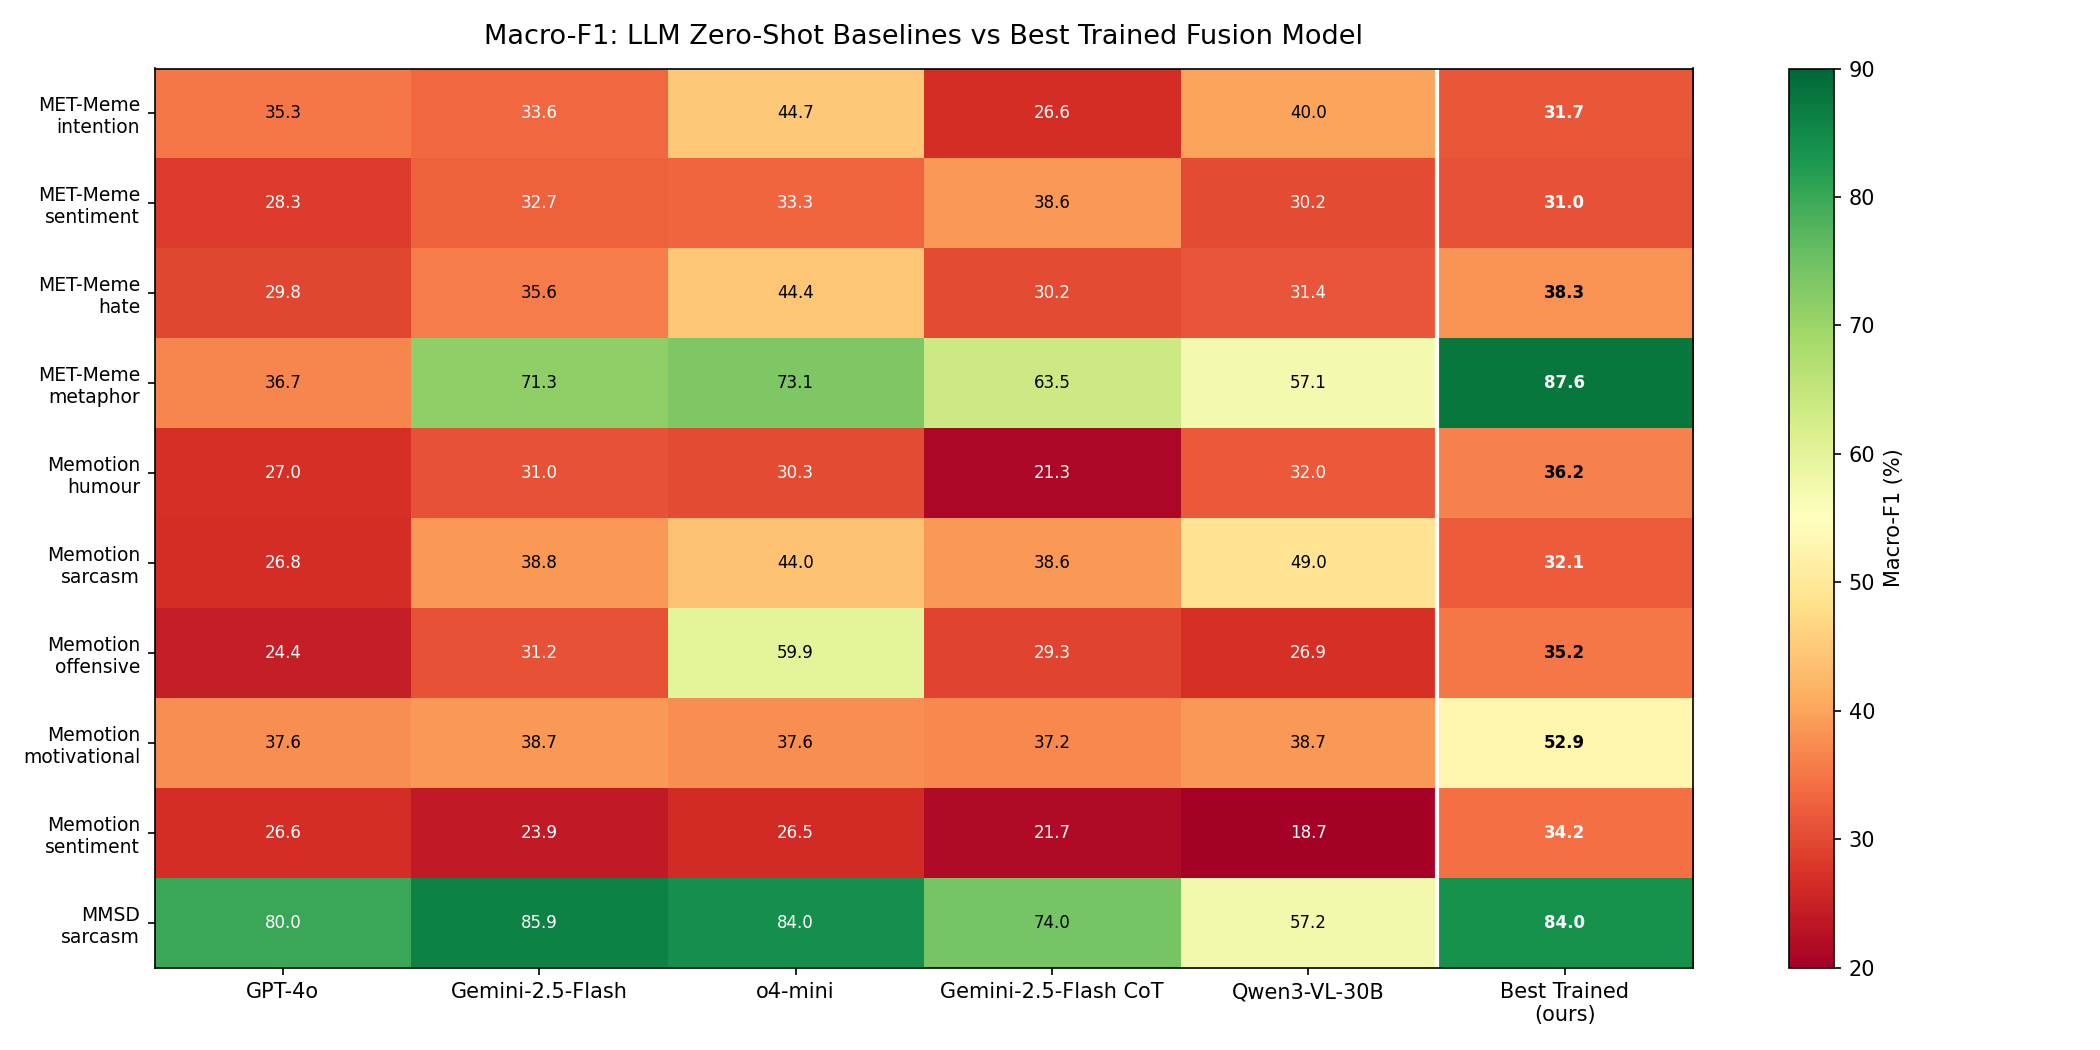
\includegraphics[width=\linewidth]{figures/llm_vs_trained_f1_heatmap.png}
  \caption{Macro-F1 gap between the best LLM zero-shot baseline and the best trained model per task.
  Green = trained model wins; red = LLM wins. Trained models dominate on structured non-literal tasks
  (metaphor, motivational, sentiment); LLMs dominate on open-ended reasoning tasks (intention, sarcasm).}
  \label{fig:llm_heatmap}
\end{figure}

% ─────────────────────────────────────────────────────────────────────────────
\section{t-SNE Visualization of Audio Embeddings}
\label{sec:tsne}

Figure~\ref{fig:tsne} shows a t-SNE projection of Emotion2Vec embeddings for all 900 audio
samples (100 memes $\times$ 9 voice settings), colored by ground-truth sentiment class.
Points cluster by sentiment rather than by voice setting, confirming that Emotion2Vec captures
semantic emotion content and is largely insensitive to surface prosodic variation (pitch, rate,
stability) introduced by different ElevenLabs voice settings.

\begin{figure}[h]
  \centering
  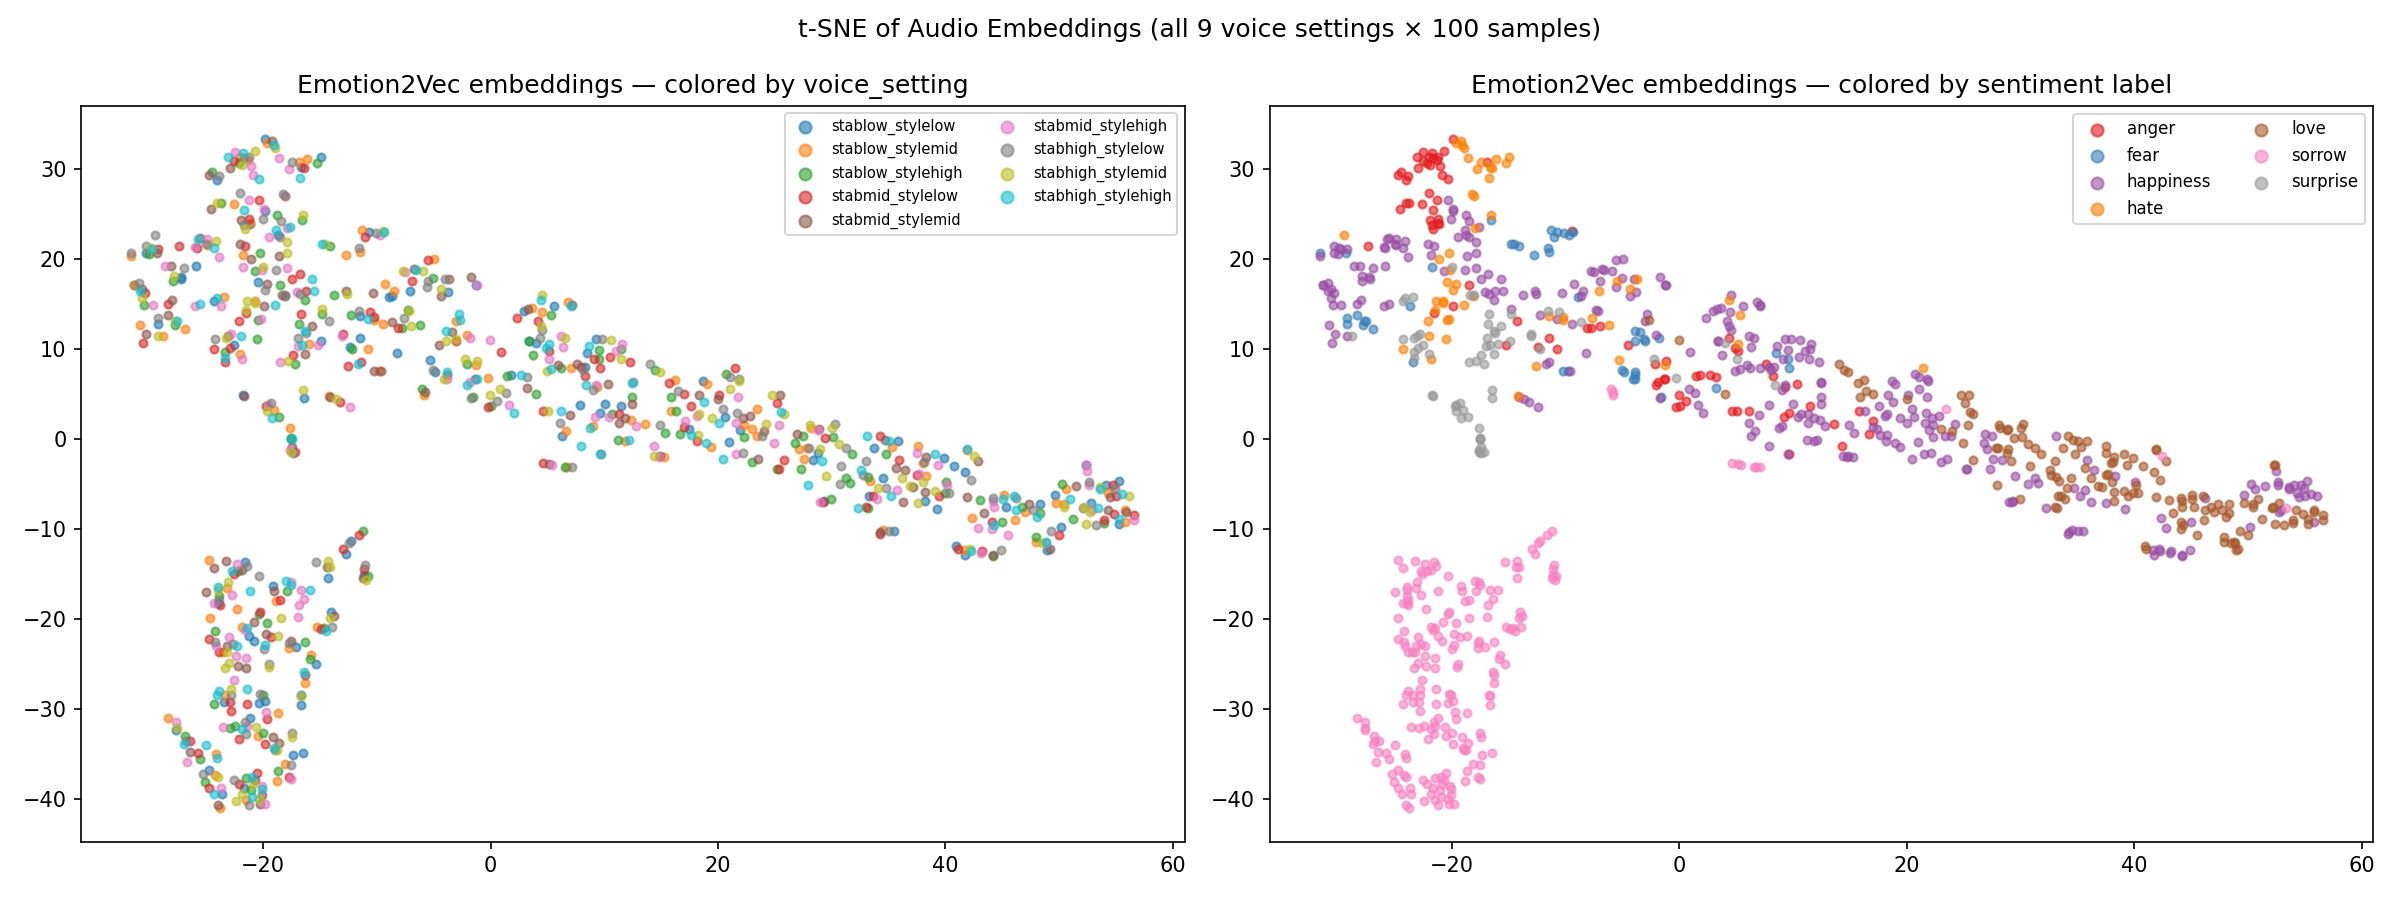
\includegraphics[width=0.85\linewidth]{figures/tsne_audio_embeddings.png}
  \caption{t-SNE of Emotion2Vec embeddings for 900 audio files (100 memes $\times$ 9 prosody settings).
  Colors indicate GT sentiment class. Clustering by sentiment rather than voice setting confirms
  Emotion2Vec's robustness to prosodic surface variation.}
  \label{fig:tsne}
\end{figure}

% ─────────────────────────────────────────────────────────────────────────────
\section{Prosody Grid Details}
\label{sec:prosody_grid}

The 9-point prosody grid used in the tri-modal alignment study spans:
\[
  \text{stability} \in \{0.2,\,0.5,\,0.8\} \;\times\; \text{style} \in \{0.2,\,0.5,\,0.8\}
\]
using ElevenLabs \texttt{voice\_settings}. All other parameters (\texttt{similarity\_boost}=0.75,
\texttt{use\_speaker\_boost}=True) are held constant. Table~\ref{tab:prosody_grid} summarizes
the intended perceptual effect of each setting combination.

\begin{table}[h]
\centering
\caption{Prosody grid: perceptual intent of each (stability, style) combination.}
\label{tab:prosody_grid}
\begin{tabular}{cc p{8cm}}
\toprule
\textbf{Stability} & \textbf{Style} & \textbf{Perceptual character} \\
\midrule
0.2 & 0.2 & Unstable, flat — inconsistent emotion, low expressiveness \\
0.2 & 0.5 & Unstable, moderate — variable rhythm, some emotional coloring \\
0.2 & 0.8 & Unstable, expressive — erratic and emotionally intense \\
0.5 & 0.2 & Neutral, flat — consistent but monotone (close to vanilla TTS) \\
0.5 & 0.5 & Balanced — moderate stability and expressiveness \\
0.5 & 0.8 & Neutral stability, high style — expressive with controlled variation \\
0.8 & 0.2 & Very stable, flat — robotic, minimal affect \\
0.8 & 0.5 & Stable, moderate — clear and measured delivery \\
0.8 & 0.8 & Stable, expressive — polished and emotionally rich \\
\bottomrule
\end{tabular}
\end{table}

% ─────────────────────────────────────────────────────────────────────────────
\section{Dataset Statistics}
\label{sec:dataset_stats}

Table~\ref{tab:dataset_stats} summarizes the dataset splits and class distributions used in
Phase~1 experiments.

\begin{table}[h]
\centering
\caption{Dataset statistics for Phase~1 benchmarks.}
\label{tab:dataset_stats}
\begin{tabular}{llcccl}
\toprule
\textbf{Dataset} & \textbf{Task} & \textbf{Train} & \textbf{Val} & \textbf{Test} & \textbf{Classes} \\
\midrule
MET-Meme  & intention    & 1{,}400 & 300 & 340 & 5 (interactive, expressive, entertaining, offensive, other) \\
MET-Meme  & sentiment    & 1{,}400 & 300 & 340 & 7 (happiness, love, anger, sorrow, fear, hate, surprise) \\
MET-Meme  & hate         & 1{,}400 & 300 & 340 & 4 (intensity levels) \\
MET-Meme  & metaphor     & 1{,}400 & 300 & 340 & 2 (binary) \\
\midrule
Memotion  & humour       & 5{,}593 & 699 & 700 & 3 \\
Memotion  & sarcasm      & 5{,}593 & 699 & 700 & 3 \\
Memotion  & offensive    & 5{,}593 & 699 & 700 & 4 \\
Memotion  & motivational & 5{,}593 & 699 & 700 & 2 \\
Memotion  & sentiment    & 5{,}593 & 699 & 700 & 3 (pos/neu/neg) \\
\midrule
MMSD 2.0  & sarcasm      & 16{,}000 & 3{,}000 & 3{,}482 & 2 (binary) \\
\bottomrule
\end{tabular}
\end{table}
